\subsection{Transformation of the Entity-Relationship Schema}


\subsubsection{Redundancy Analysis}
The schema does not contain any cycle of entities.
\subsubsection{Choice of Principal Identifiers}
The main identifiers comply with the selection criteria.

\subsection{Analysis of Database Load}
Since there is not any derived attribute in the provided ER-Schema, we provide the load analysis as if the Book entity had the number of copies as derived attribute. Consider the following two operations that involve the redundant attribute 'numberofcopies': \newline
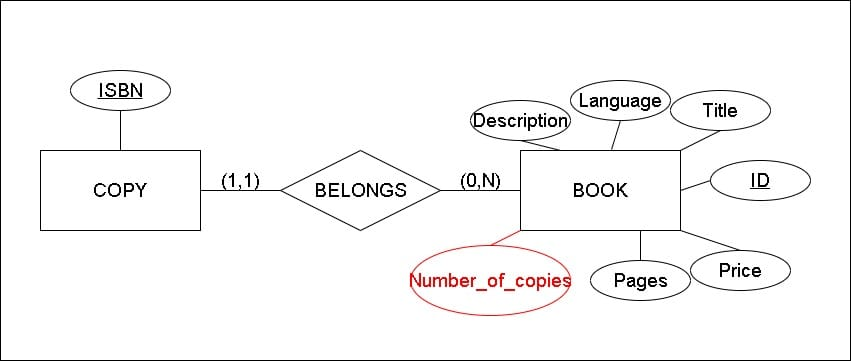
\includegraphics[scale=0.4]{sections/Relation.jpeg} \newline
O1 - Insert new copy : store a new copy together with its book ID. 

O2 - Print data about a book: print all the data about a book, including the number of copies 

O3 - Summarise data about all the books: summarise all the data about all the books, including the number of copies 
In Table 3 the two operations are described.
Table 3: Operations description and frequency 
\begin{center}
\begin{tabular}{|r|r|r|r|}
\hline

    Operation & Description & Frequency & Type\\\hline
   
O1 : Add new copy & store a new copy together \\ &with book ID  & 100/day & Online \\\hline
O2 : Print data about a book & print all the data about a book, \\ &including the number of copies  & 2/day  & Online \\\hline
O3 : Summarize data about \\ all the books & summarize all the data about\\ & all the books, \\&including the number of copies  &1/week   & Batch \\\hline

   
\end{tabular}
\end{center}



In Table  4 we report the access/volume data related to O1 with redundancy. The Book entity has a read access to get the current value for "numberofcopies" attribute, and a write access to update this value. 

Table 4: Access/volume Table for Operation 1 with redundancy .\\

\begin{center}
\begin{tabular}{|r|r|r|r|r|}
\hline
\multicolumn{5}{|l|}{O1}\\\hline
    Concept & Construct & Access & Type & Average 
    Access\\\hline
    {Copy} &  {Entity} &  {1}  & {W}  & {1x100x2=200 }\\\hline
      {Belong } &  {Relationship} &  {1}  & {W}  & {1x100x2=200 }\\\hline
    {Book } &  {Entity} &  {1}  & {R}  & {1x100x1=100 }\\\hline
     {Book } &  {Entity} &  {1}  & {W}  & {1x100x2=200 }\\\hline

    \multicolumn{4}{|l}{Total Access}&\multicolumn{1}{|l|}{700}\\\hline
\end{tabular}
\end{center}
In Table  5 we report the access/volume data related to O2 with redundancy. The presence of redundancy allows us to perform one access to the Book entity to get all the required information. 

Table 5: Access/volume Table for Operation 2 with redundancy 
\begin{center}
\begin{tabular}{|r|r|r|r|r|}
\hline
\multicolumn{5}{|l|}{O2}\\\hline
    Concept & Construct & Access & Type & Average 
    Access\\\hline
      {Book } &  {Entity} &  {1}  & {R}  & {1x2x1=2 }\\\hline

    \multicolumn{4}{|l}{Total Access}&\multicolumn{1}{|l|}{2}\\\hline
\end{tabular}
\end{center}
In Table  6 we report the access/volume data related to O1 without redundancy. In this case we have to consider the insertion of a new instance in copy, and the insertion of a new instance in belong  to store the book the copy joined. 

Table 6: Access/volume Table for Operation 1 without redundancy 

\begin{center}
\begin{tabular}{|r|r|r|r|r|}
\hline
\multicolumn{5}{|l|}{O1}\\\hline
    Concept & Construct & Access & Type & Average Access\\\hline
{Copy} &  {Entity} &  {1}  & {W}  & {1x100x2=200 }\\\hline
      {Belong } &  {Relationship} &  {1}  & {W}  & {1x100x2=200 }\\\hline

    \multicolumn{4}{|l}{Total Access}&\multicolumn{1}{|l|}{400}\\\hline
\end{tabular}
\end{center}
In Table  7 we report the access/volume data related to O2 without redundancy. We considered 20 copies on average for each book. 

Table 7: Access/volume Table for Operation 2 without redundancy 

\begin{center}
\begin{tabular}{|r|r|r|r|r|}
\hline
\multicolumn{5}{|l|}{O2}\\\hline

    Concept & Construct & Access & Type & Average Access\\\hline
         {Book } &  {Entity} &  {1}  & {R}  & {1x2x1=2  }\\\hline
      {Belong } &  {Relationship} &  {20}  & {R}  & {20x2x1=40 }\\\hline

   \multicolumn{4}{|l|}{Total Access}&\multicolumn{1}{|l|}{42}\\\hline
\end{tabular}
\end{center}
In Table  8 we report the final access count with and without redundancy. According to the obtained results, removing the redundant attribute from the group entity improves the load analysis. 

Table 8: Comparison of the number of accesses for each operation 


\begin{center}
\begin{tabular}{|r|r|r|}
\hline
     Operation & With Redundancy & Without Redundancy\\\hline
    O1 & 700 & 400  \\\hline
    O2 & 2 & 42 \\\hline
    Total Access/Week & 702 & 442 \\\hline
\end{tabular}
\end{center}

\subsection{Relational Schema}
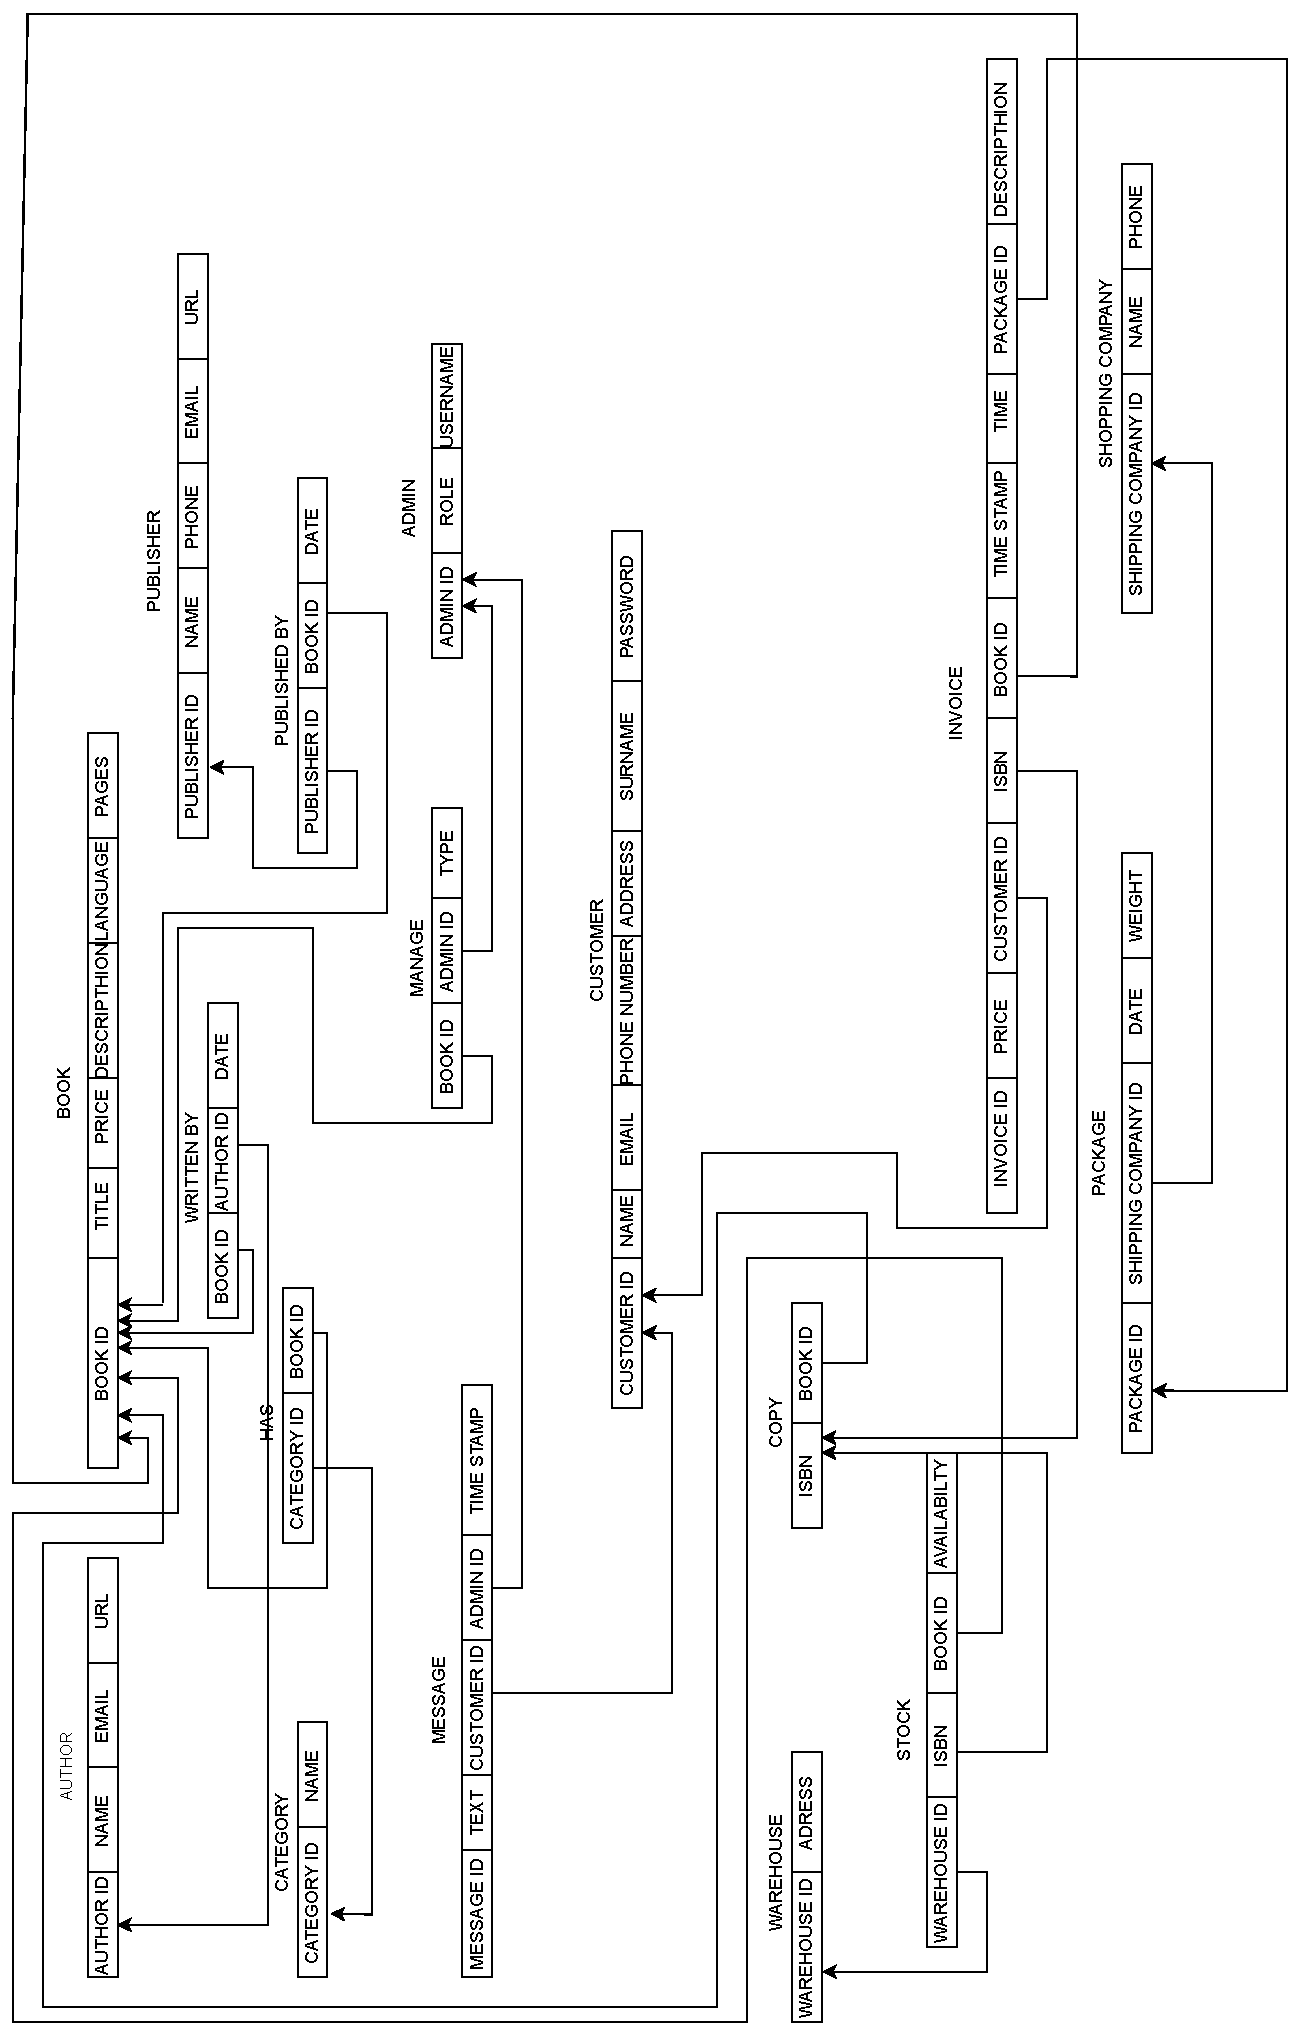
\includepdf[scale=0.9]{sections/Relational_sch.pdf}

\subsection{Data Dictionary}

\begin{longtable}{|p{.15\columnwidth}|p{.15\columnwidth} |p{.30\columnwidth}|p{.10\columnwidth}|p{.20\columnwidth} |} 
\hline
\textbf{Relation} & \textbf{Attribute} & \textbf{Description} & \textbf{Domain} & \textbf{Constraints} \\\hline


\multirow{7}{*}{Book} 
& Book ID & Book identifier & serial  & Primary Key \\\cline{2-5}
& Title &title of the book &text  & Not Null\\\cline{2-5}
& Price & the cost of the book &float& Not Null\\\cline{2-5}
& Pages& the number of pages of the book &integer & Not Null \\\cline{2-5}
& Language&the language of the book in which the book is written to &text & Not Null\\\cline{2-5}
& Description &a brief information about the book & text & \\\cline{2-5}
& ISBN &the physical book which is held in the warehouse and will be delivered to the customer & serial & Foreign Key to Copy\\\hline

\multirow{4}{*}{Author} & Author
ID & author identifier &serial & Primary Key\\\cline{2-5}
& Name &Full name of the author &text & Not Null\\\cline{2-5}
& URl & the link to the personal webpage of the author &text& \\\cline{2-5}
& Email & email address of the author &text & \\\hline


\multirow{5}{*}{Publisher} & Publisher ID
&publisher identifier &serial & Primary Key \\\cline{2-5}
& Name & the name of the publishing company &text  &Not Null \\\cline{2-5}
& URL & publisher website link &text  & \\\cline{2-5}
& Phone & the phone number to access the publisher &integer &Not Null \\\cline{2-5}
& Email &the publisher email &text &Not Null \\\hline


\multirow{2}{*}{Category} & Category ID & identifier of the category &serial & Primary Key\\\cline{2-5}
& Name & the name of the category &text & Not Null \\\hline


\multirow{5}{*}{Copy} & ISBN & The International Standard Book Number is a numeric commercial book identifier that is intended to be unique & serial & Primary Key\\\cline{2-5}

&Book ID & Book identifier & serial  & Foreign Key to Book, Not Null\\\hline

\multirow{4}{*}{ShippingCompany} & Shipping Company ID &identifier of the company & serial& Primary Key\\\cline{2-5}
& Name & name of the company &text & Not Null\\\cline{2-5}
& Phone &phone number of the company &integer &  Not Null\\\hline

\multirow{10}{*}{Customer} & Customer
ID & identifier of the customer &serial & Primary Key\\\cline{2-5}
& Name & first name of the customer &text & Not Null\\\cline{2-5}
& Address & the address of the customer which the books will be delivered to &text  & Not Null\\\cline{2-5}
& Email & email of the customer which is used also to log in &text & Not Null \\\cline{2-5}
& Phone & the phone number of the customer &integer & Not Null\\\cline{2-5}
& surname & the last name of the customer &text  & Not Null \\\cline{2-5}
& Password & the password which is used to login to the system & text & Not Null \\\hline

\multirow{10}{*}{Invoice} & Invoice ID & identifier of the invoice &serial & Primary Key\\\cline{2-5}
& Price & the price of the purchase & float & Not Null \\\cline{2-5}
& Description & the description about the purchase &text & \\\cline{2-5}
& Customer
ID & identifier of the customer &serial & Foreign Key to Customer, Not Null\\\cline{2-5}
&ISBN & The International Standard Book Number is a numeric commercial book identifier that is intended to be unique & serial  & Foreign Key to Copy, Not Null \\\cline{2-5}
& Book ID & Book identifier & serial  & Foreign Key to Book, Not Null \\\cline{2-5}
& Timestamp & the time in which the purchase took place at &timestamp & Not Null \\\hline

\multirow{5}{*}{Package} & Package ID & identifier of the package &serial & Primary Key\\\cline{2-5}
& weight & the weight of the package to calculate the cost of delivery &float & Not Null\\\cline{2-5}
&Shipping Company ID &identifier of the company & serial& Foreign Key to Shipping Company, Not Null  \\\cline{2-5}
& Date & date when the shipping has started & text & Not Null  \\\hline

\multirow{2}{*}{Warehouse} & Warehouse ID &Identifier of the warehouse &serial & Primary Key \\\cline{2-5}
&address & the address of where the warehouse is located &text & Not Null \\\hline

\multirow{4}{*}{\texttt{Written\_by} } & Book ID & Book identifier & serial  & Foreign Key to Book, Not Null\\\cline{2-5}
& Author
ID & author identifier &serial & Foreign Key to Author, Not Null \\\cline{2-5}
& Date & The date in which the book was written by author & date & \\\hline

\multirow{4}{*}{\texttt{Published\_by}} & Book ID & Book identifier & serial  & Foreign Key to Book, Not Null\\\cline{2-5}
& Publisher ID
&publisher identifier &serial & Foreign Key to Publisher, Not Null\\\cline{2-5}
& Date & The date in which the book was published by publish & date & Not Null \\\hline

\multirow{2}{*}{Has} & Category ID & identifier of the category &serial & Foreign Key to Category, Not Null\\\cline{2-5}
& Book ID & Book identifier & serial  & Foreign Key to Book \\\hline

\multirow{1}{*}{Admin} & Admin ID &identifier of the admin &serial & Primary Key\\\cline{2-5}
& Role & the role of the admin in the system,they can be in Support department or the ones who add or delete the books, change prices or write description of the books(Manage department) &text & Not Null\\\cline{2-5}
& username & the username to login &text &Not Null \\\cline{2-5}
& password & the pass word to login &text & Not Null\\\hline

\multirow{4}{*}{Manage} & Admin ID &identifier of the admin &serial & Foreign Key to Manage\\\cline{2-5}
& Book ID & Book identifier & serial  & Foreign Key to Book, Not Null \\\cline{2-5}
& Type &it shows the type of the management,it could be add,remove,modify &text & Not Null\\\hline

\multirow{4}{*}{Message} 
& ID &identifier of the message &serial & Primary key\\\cline{2-5}
& Text &the text of the message written by admin and customer & text & Not Null\\\cline{2-5}
& Admin ID &identifier of the admin &serial & Foreign Key to Admin, Not Null\\\cline{2-5}
& Customer
ID & identifier of the customer &serial & Foreign Key to Customer, Not Null\\\cline{2-5}
& timestamp & the time of the chat took place at & timestamp & Not Null  \\\hline

\multirow{4}{*}{Stock} & Warehouse ID &Identifier of the warehouse &serial &  Primary Key\\\cline{2-5}
& ISBN & The International Standard Book Number is a numeric commercial book identifier that is intended to be unique & serial & Foreign Key to Copy, Not Null\\\cline{2-5}
& Book ID & Book identifier & serial  & Foreign Key to Book, Not Null\\\cline{2-5}
& availability & a boolean which tells us if a book is available or not & bool & Not Null\\\hline
\end{longtable}

\subsection{External Constraints}
\begin{itemize}
        
        \item The admin can changes the book(add,delete,change price,change description) depending on his Role: we have to check the manageType and adminRole attributes to be compatible.
        \item The customer can only purchase the book which is available in the warehouses: a copy should be purchased if it's stockAvalability is TRUE.
        \item The package should be shipped by the shipper due to time limit that is announced in the website(for example it says in 3 working days it will be delivered): the placedTime and shipped\_ byDate should not violate this limit.
        \item The customer should only chat to the admin whose Role is Support: the adminRole must be Support.
    \end{itemize}